\section{Technische Umsetzung des Datenflusses zur Anzeige}
%\textcolor{red}{Beschreibungd des Tools}}
\label{ch:IST-Zustand:sec:Datenfluss}

% ******************************************************
%       Tool
% ******************************************************
Jeder dieser Tests wird gruppiert durch einen Job durchgeführt. Sobald die Testsammlungen eines Tools durchgelaufen sind, werden deren Ergebnisse in eine Textdatei geschrieben (s. \autoref{fig:alt_Datenfluss}).
Das Tool für die Er\-geb\-nis\-an\-zeige ist ein selbstgeschriebenes Tool und eine Art Vorstufe eines Dash\-boards. Das Skript zur Ausführung dieser Oberfläche überprüft, ob alle Ergebnisse valide sind, abhängig davon können weitere Tests gestartet werden.
Das Tool liest die Textdatei mit den Ergebnissen aus, bereitet die Daten auf und erzeugt jeweils eine Übersichtsseite pro Version bzw. Anwendungsfall.

%- selbstgeschrieben
%- pro Version eine Übersichtsseite
%- das scresult.exe überprüft, ob das Gesamtergebnis ok/not ok ist
%--> daraufhin Entscheidung für weitere Tests oder nicht

%Selbstgeschrieben:
% Hintergrund: Textfile - wo die Ergebnisse reingeschrieben werden
% verschiedene Testtools schreiben seine Ergebnisse in das File (der Job / das Script davon)
%- Scresult: zieht sich die Daten aus dem File und bereitet diese auf
% --> formatierten / strukturieren für die Oberfläche

% ******************************************************
%       Datenfluss
% ******************************************************
\begin{figure}[H]
    \centering
    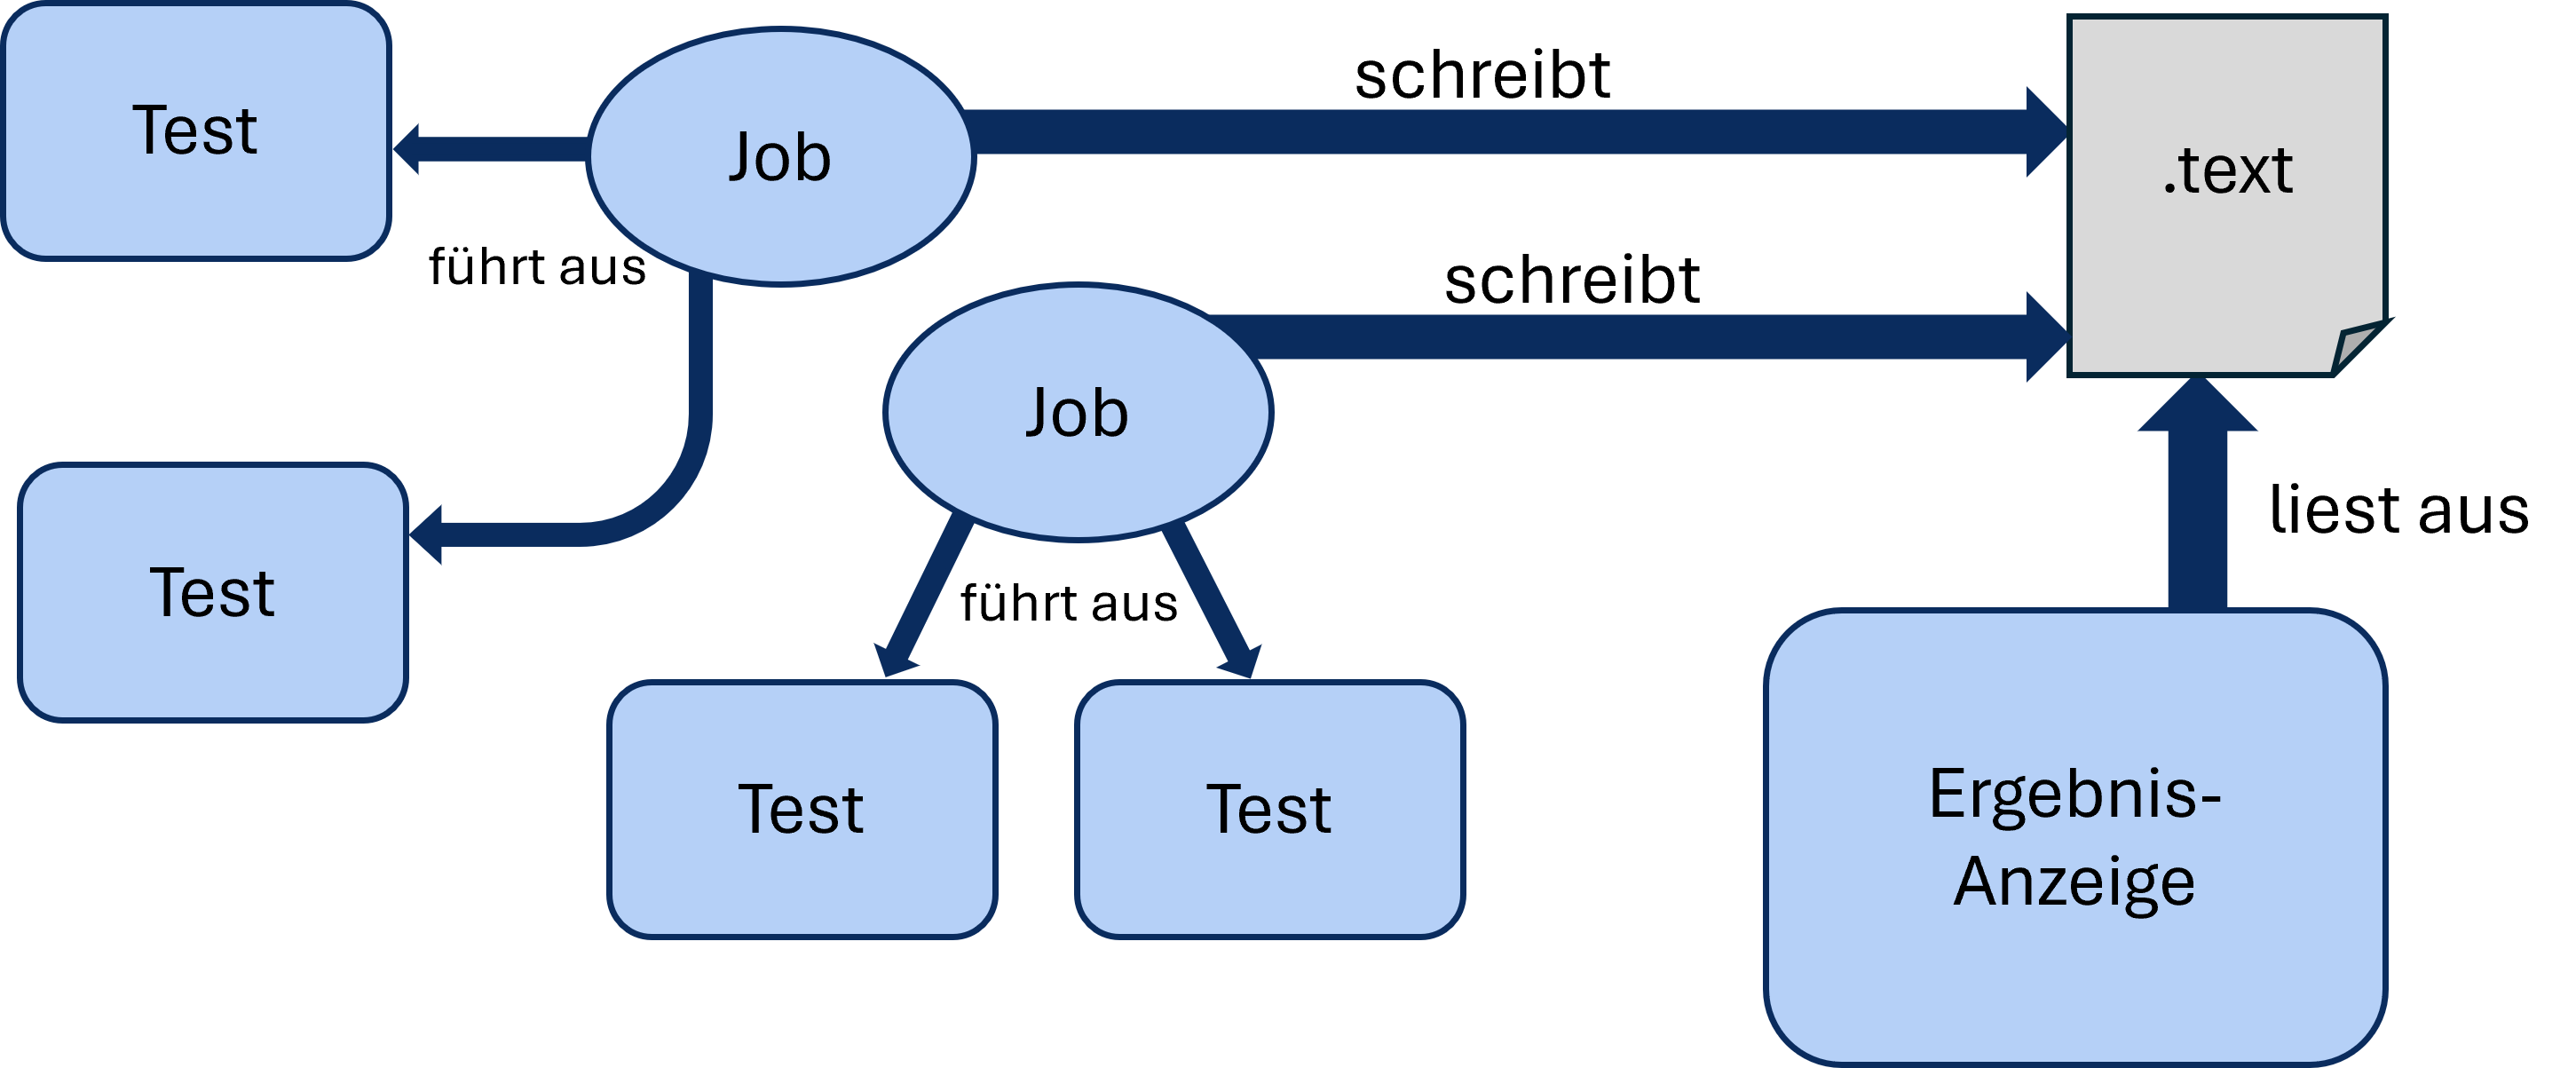
\includegraphics[width=1\linewidth]{Dashboard/Daten_Kontrollsequenz_IST.png}
    \caption{Kontrollsequenz des Datenflusses vom ausgeführten Test zur Ergebnisanzeige}
    \label{fig:alt_Datenfluss}
\end{figure}

%\textcolor{red}{JenkinsJob > schreibt Ergebnis auf Oberfläche > cmd-Output auch abrufbar}
